\documentclass{article}
\usepackage{listings}
\usepackage{graphicx}
\usepackage{adjustbox}

\begin{document}
\begin{enumerate}
\item A stradegy would be to sort the tasks by deadlines, then pick the task with the earliest deadline and remove it from your overall selection, as well as remove any tasks that cannot be finished if the picked task is removed. Continue doing this until there are no more tasks that haven't been picked. This stradegy works because the task with the earliest deadline is always picked first, therefore maximizing the amount of tasks that can be performed.
\item \begin{enumerate}
	\item \begin{minipage}[t]{\linewidth}
          \raggedright
          \adjustbox{valign=t}{%
            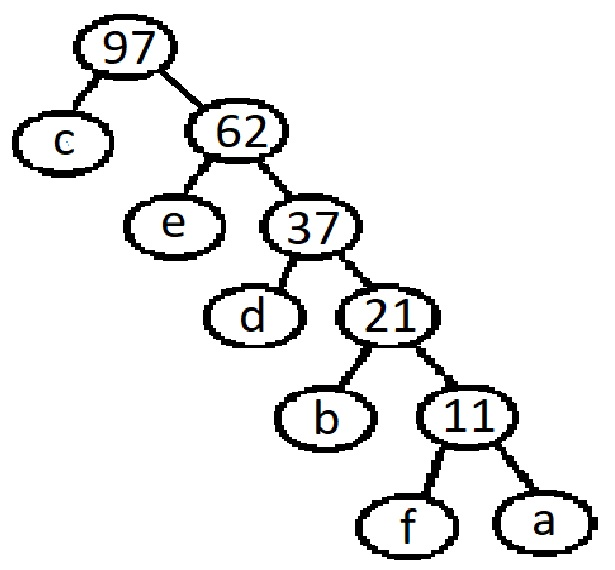
\includegraphics[width=.8\linewidth]{tree.jpg}%
         	 }
	\end{minipage}
	\item a: 11111  b: 1110  c: 0  d: 110  e: 10
	\item \begin{math} 5*2+4*10+1*35+3*16+2*25=183 \mbox{ bits}
		\end{math}
	\item \begin{math} \mbox{raw text size}=8*2+8*10+8*35+8*16+8*25+8*9=776\mbox{ bits}\\
		\mbox{compression ratio}=183/776=0.2358
		\end{math}
	\end{enumerate}
\item \begin{enumerate}
	\item Modify Dijkstra's algorithm such that once the destination has been visited, a counter increases from 0 to 1 and the weight of that route is saved. The code then backtracks 				recursively, checking all possible routes that have not been seen before and comparing their weights to the saved weight. If the weights are equal, the counter increases. Once the 			backtracking is complete, the counter number is returned.
	\item Create an array that is meant to hold all minimum SUB-route weights. Iteratively walk through the graph starting from (0,0) and ending at (M,N), switching and saving routes in the 			array if the weight of the current route so far is the smallest possible. Once (M,N) is reached, start again from (0,0) and reuse all the subroutes saved in the array except for the last one, 		then check to see if there is another route to (M,N) that has the same weight as the previous one. If there is, set a counter to 2 and repeat the process again and again using 1 less 			subroute from the array each time, increasing the counter if the condition is met. The time cost of this algorithm would be \begin{math}O((MN)^2)\end{math} because in the worst case, 			every vertex will be visited M*N times.
	\end{enumerate}
\item \begin{enumerate}
	\item (1) Given an array of numbers where each element represents the max number of jumps that can be made forward from that element, for each array element, count number of ways 		jumps can be made from that element to reach the end of the array. \\(2) Given two strings ‘str1’ and ‘str2’ of size m and n respectively, remove/delete and insert the minimum number of 			characters from/in str1 so as to transform it into str2.\\ (3) Given a string containing characters as integers only, delete all characters of this string in a minimum number of steps where in 			one step you can delete the substring which is a palindrome.
	\item (1) The main idea is to traverse through the array starting at the first element and find all other elements reachable from that first element, then determine the minimum number of 			jumps needed to reach end from the elements reachable from first. After that, the minimum number of jumps to reach end from first can be calculated using the number previously 				determined. A recursive call can be used at every element reachable from the first element to get the minimum number of jumps needed at each step.\\
	(2) unfinished\\
	(3) The main idea is to find all substrings greater than one character in the string that are palindromes, then remove them in such a way so that the entire string is deleted in as little steps 		as possible. The recursive calls would be executed after each palindrome is found, accounting for cases in which parts of some palindromes are included inside other palindromes.
	\item (1) The recursive-based idea revisits and resolves the same problems several times: finding the minimum number of jumps needed to reach the end from elements reachable from the 		first element. \\
	(2) unfinished\\
	(3) Recursively, the same palindrome could be found several times before it is recorded, therefore identical problems are repeatedly solved again and again.
	\item (1) Dynamic programming works because an array can be created to store the minimum jumps needed to reach a given element from the first element. This array can be reused over 		and over instead of solving the same problems multiple times.\\
	(2) unfinished\\
	(3) Dynamic programming works because each palindrome, including palindromes partially or completely inside other palindromes) is saved in a local array and can be reused if visited again.
	\item (1) http://www.geeksforgeeks.org/minimum-number-of-jumps-to-reach-end-of-a-given-array/ \\
	(2) http://www.geeksforgeeks.org/minimum-number-deletions-insertions-transform-one-string-another/ \\
	(3) http://www.geeksforgeeks.org/minimum-steps-to-delete-a-string-after-repeated-deletion-of-palindrome-substrings/
	\end{enumerate}
\end{enumerate}
\end{document}
